%% LyX 2.2.3 created this file.  For more info, see http://www.lyx.org/.
%% Do not edit unless you really know what you are doing.
\documentclass[oneside,english]{extbook}
\usepackage{lmodern}
\renewcommand{\sfdefault}{lmss}
\renewcommand{\ttdefault}{lmtt}
\usepackage[T1]{fontenc}
\usepackage[latin9]{inputenc}
\usepackage{geometry}
\geometry{verbose,tmargin=25mm,bmargin=25mm,lmargin=25mm,rmargin=25mm}
\pagestyle{plain}
\setcounter{secnumdepth}{3}
\setcounter{tocdepth}{3}
\setlength{\parindent}{0bp}
\usepackage{babel}
\usepackage{float}
\usepackage{graphicx}
\usepackage{setspace}
\onehalfspacing
\usepackage[unicode=true,pdfusetitle,
 bookmarks=true,bookmarksnumbered=false,bookmarksopen=false,
 breaklinks=false,pdfborder={0 0 1},backref=false,colorlinks=false]
 {hyperref}

\makeatletter
%%%%%%%%%%%%%%%%%%%%%%%%%%%%%% User specified LaTeX commands.
\usepackage{amssymb}
\usepackage{color}
\usepackage{listings}
\definecolor{hellgelb}{rgb}{1,1,0.85}
\definecolor{colKeys}{rgb}{0,0,1}
\definecolor{colIdentifier}{rgb}{0,0,0}
\definecolor{colComments}{rgb}{1,0,0}
\definecolor{colString}{rgb}{0,0.5,0}
\lstset{
      language=Matlab,
      float=hbp,
      basicstyle=\footnotesize\ttfamily,
      identifierstyle=\color{colIdentifier},
      keywordstyle=\color{colKeys},
      stringstyle=\color{colString},
      commentstyle=\itshape\color{colComments},
      columns=fixed,
      tabsize=4,
      frame=single,
      framerule=1pt,
      extendedchars=true,
      showspaces=false,
      showstringspaces=false,
      numbers=left,
      numberstyle=\tiny\ttfamily,
      numbersep=1em,
      breaklines=true,
      breakindent=10pt,
      backgroundcolor=\color{hellgelb},
      breakautoindent=true,
      captionpos=t,
      xleftmargin=1em,
      xrightmargin=\fboxsep
}
\usepackage{lscape}
\usepackage{amsmath}
\usepackage{mathtools}
\usepackage{pifont}
\usepackage{color}
\usepackage{accents}

\delimitershortfall=-1pt
\let\Right\right
\let\Left\left
\makeatletter
\def\right#1{\Right#1\@ifnextchar){\!\right}{}}
\def\left#1{\Left#1\@ifnextchar({\!\left}{}}
\makeatother

\makeatother

\begin{document}
\pagenumbering{gobble}

\begin{figure}[H]
\centering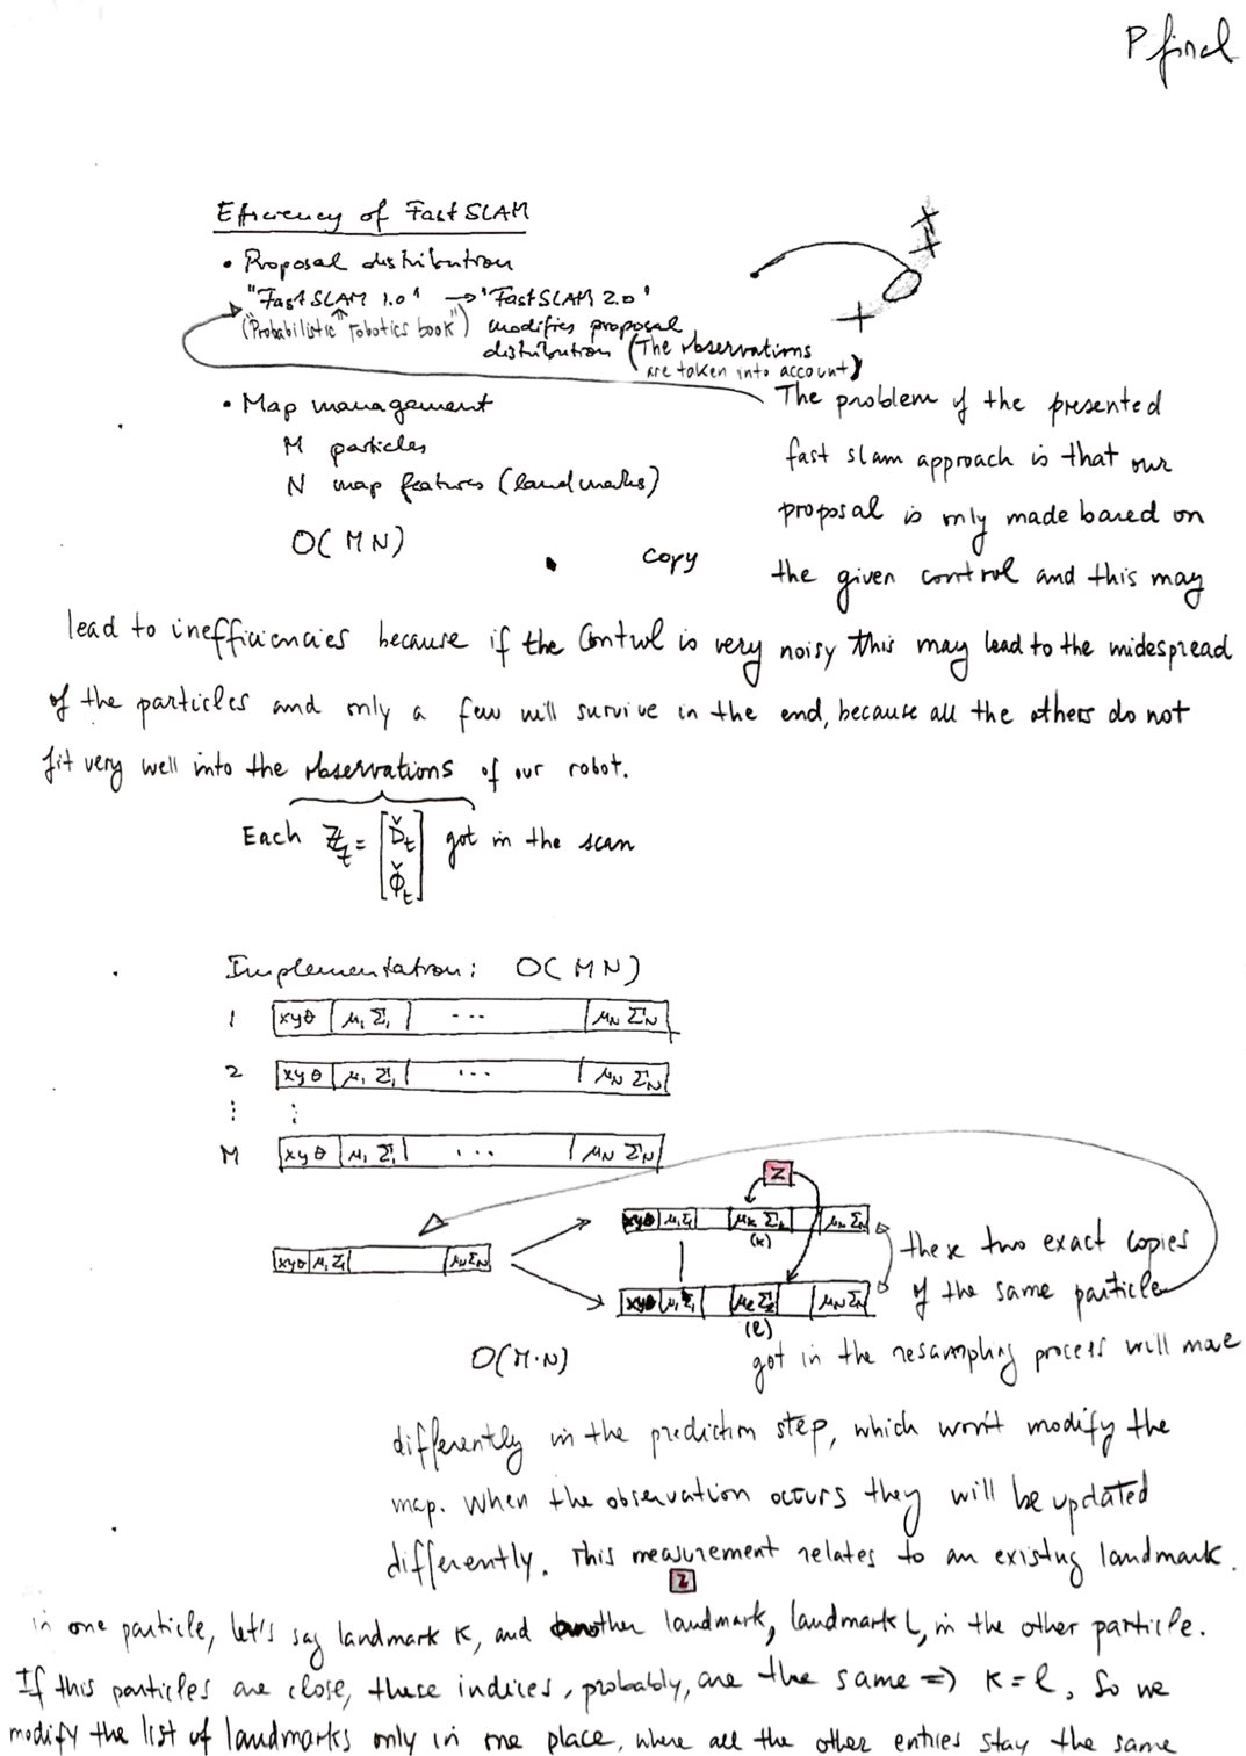
\includegraphics[clip,width=0.99\textwidth,height=0.99\textheight,keepaspectratio]{../FIGURES/fig82}
\end{figure}

\begin{figure}[H]
\centering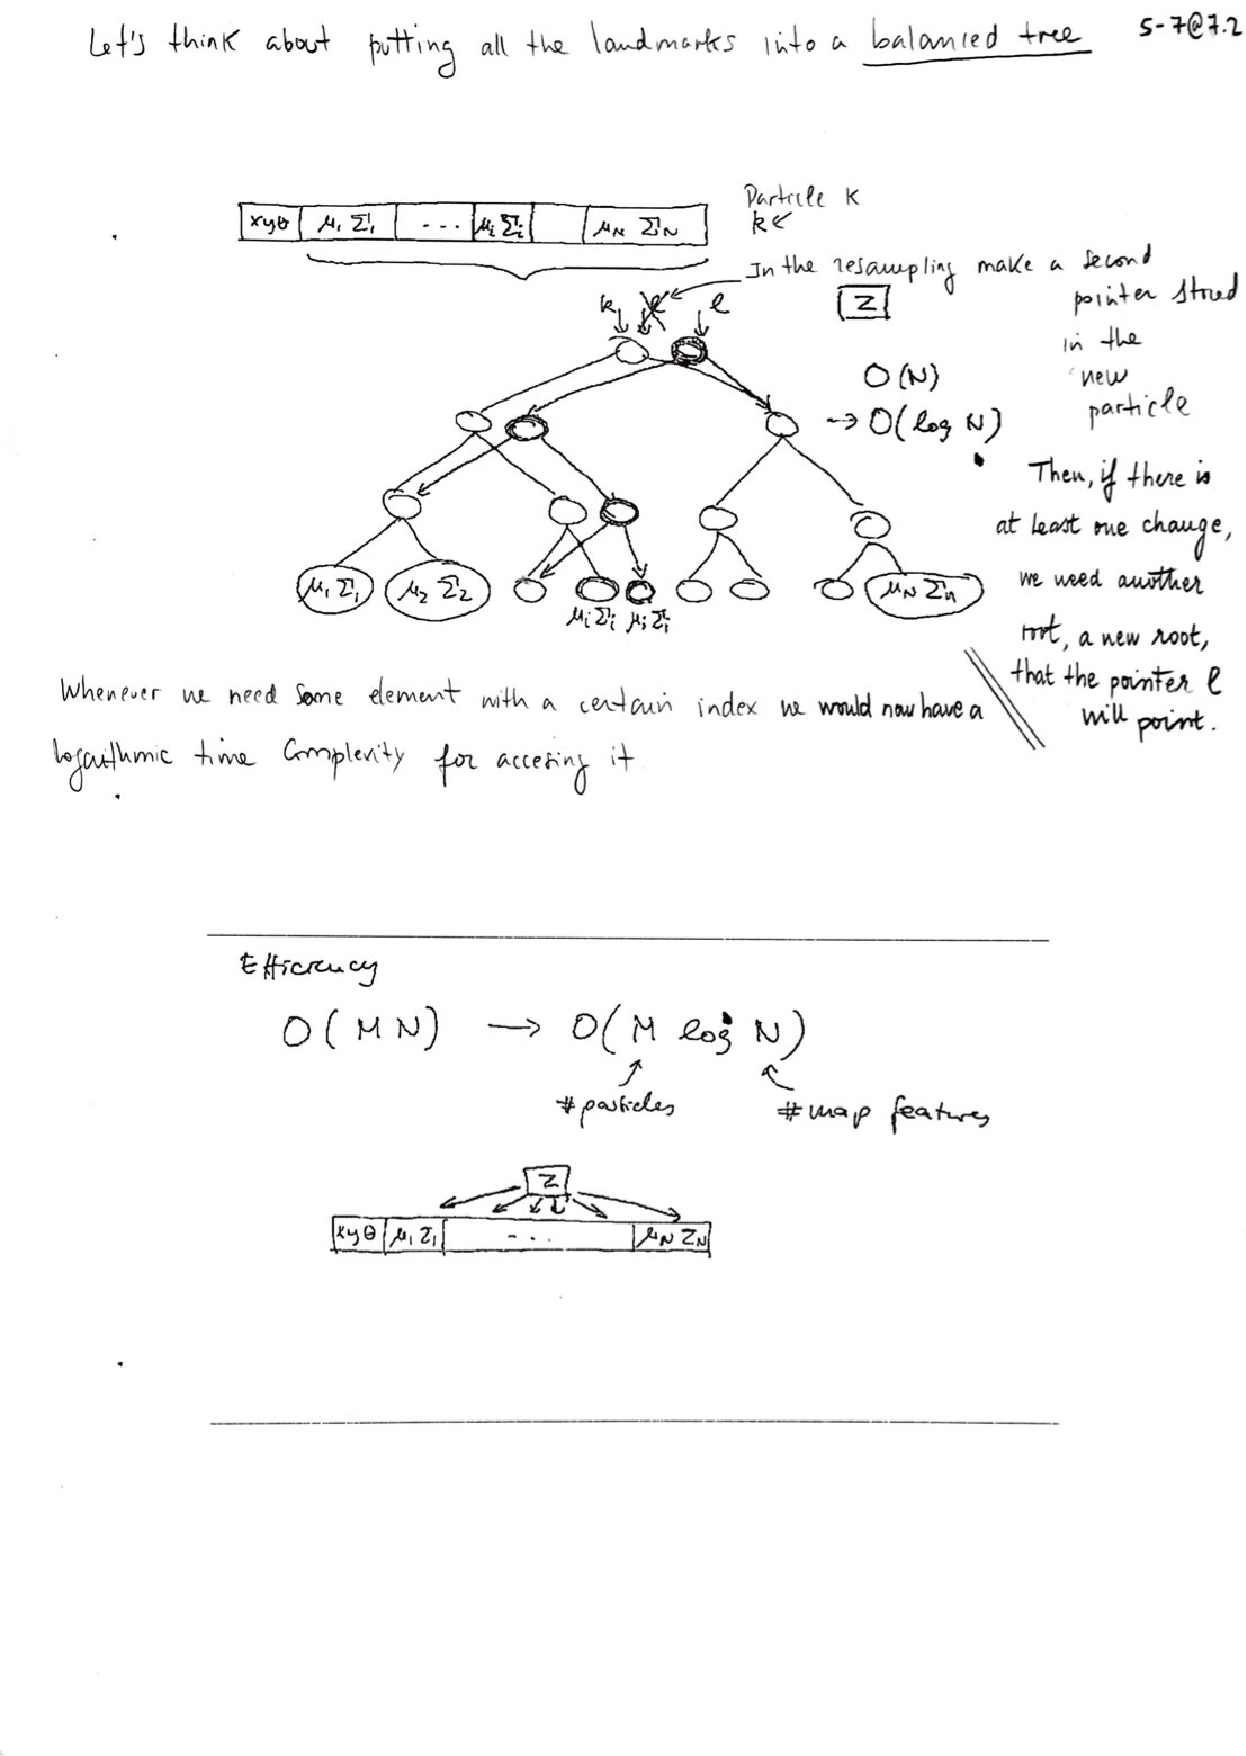
\includegraphics[clip,width=1\textwidth,height=1\textheight,keepaspectratio]{../FIGURES/fig84}
\end{figure}

\begin{figure}[H]
\centering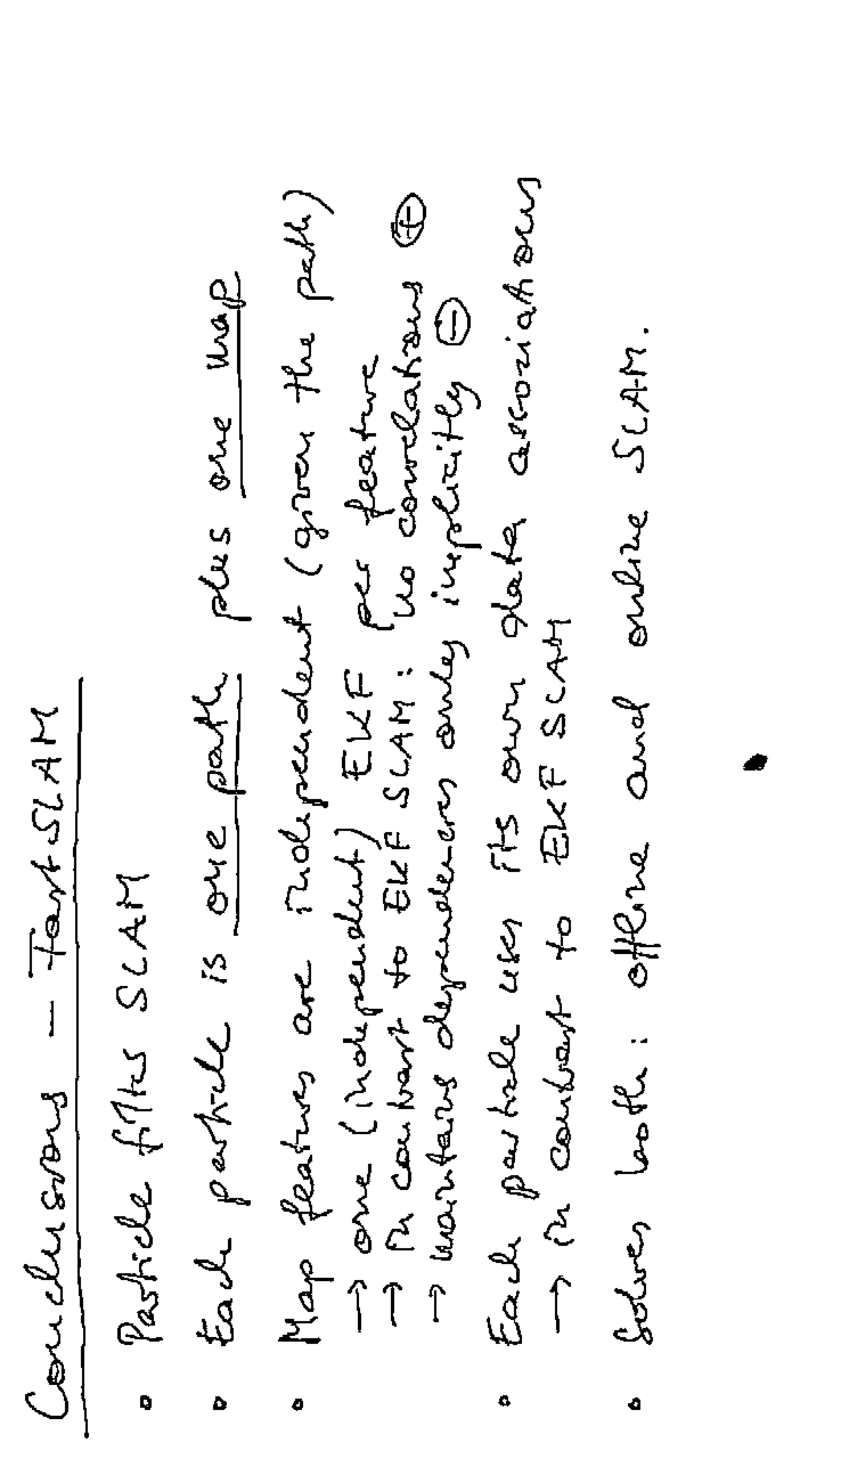
\includegraphics[clip,width=1\textwidth,height=1\textheight,keepaspectratio]{../FIGURES/fig86}
\end{figure}

\end{document}
